\documentclass[a4paper,12pt,bibliography=totoc, listof=totoc,titlepage]{scrreprt}
\usepackage[ngerman]{babel}
\usepackage[utf8]{inputenc}
\usepackage[left=3cm,right=2.5cm,top=2.5cm,bottom=2.5cm]{geometry}
\usepackage[onehalfspacing]{setspace}
\renewcommand{\arraystretch}{1.5}
\usepackage{graphicx}
\usepackage{color}
\usepackage[dvipsnames,usenames,dvipsnames,table,xcdraw]{xcolor}
\usepackage[toc,page]{appendix}
\usepackage[printonlyused]{acronym}
%\usepackage[scaled]{berasans}
%\renewcommand*\familydefault{\sfdefault}  %% Only if the base font of the document is to be sans serif
%\usepackage[T1]{fontenc}

% Absatz-Einstellungen
\setlength{\parindent}{15pt} % Einrücken
\setlength{\parskip}{6pt}  % Horizontaler Abstand

\usepackage{subcaption}
\usepackage{graphicx} % omit 'demo' for real document
  
\usepackage[hyphens]{url}
\usepackage[hidelinks]{hyperref}
\setlength {\marginparwidth }{2cm}
\usepackage{todonotes}
\usepackage{amsmath}
\usepackage{cancel}

% Kommentare mit \begin{comment}
\usepackage{verbatim}

\usepackage{multirow}

\newcommand*\justify{%
  \fontdimen2\font=0.4em% interword space
  \fontdimen3\font=0.2em% interword stretch
  \fontdimen4\font=0.1em% interword shrink
  \fontdimen7\font=0.1em% extra space
  \hyphenchar\font=`\-% allowing hyphenation
}

\newcommand{\code}[1]{\texttt{\justify{#1}}}
%\usepackage{tocloft}

%Boxfehler
\hbadness=1000000

% Hurenkinder und Schusterjungen verhindern
\clubpenalties 4 10000 10000 1000 1000
\widowpenalties 4 10000 10000 1000 1000
\displaywidowpenalty=10000

% Listings
\usepackage{listings}
\lstset{
   breaklines=true,
   captionpos=t,
   basicstyle=\scriptsize\ttfamily,
   keywordstyle=\bfseries\ttfamily\color{orange},
   stringstyle=\color{green}\ttfamily,
   commentstyle=\color{gray}\ttfamily,
   emph={square}, 
   emphstyle=\color{blue}\texttt,
   emph={[2]root,base},
   emphstyle={[2]\color{yac}\texttt},
   showstringspaces=false,
   flexiblecolumns=false,
   tabsize=2,
   numbers=left,
   numberstyle=\tiny,
   numberblanklines=false,
   stepnumber=1,
   numbersep=10pt,
   xleftmargin=15pt
 }

% Zitierstil
%\usepackage[style=authoryear,citestyle=authoryear,natbib=true]{biblatex}
%\bibliography{Thesis.bib}
\usepackage[round]{natbib}
\bibliographystyle{hcu}

\begin{document}
\pagenumbering{Roman}
\begin{titlepage}
\begin{center}
\renewcommand{\arraystretch}{0.7}
\begin{tabular}{lr}
\begin{tabular}{l}

\includegraphics[width=0.35\textwidth]{img/hculogo_grau.png}
\end{tabular} \hspace{1.2cm} &
\begin{tabular}{r}
Universität für \\Baukunst und Metropolenentwicklung\\
Henning-Voscherau-Platz 1\\
20457 Hamburg\\
\end{tabular}
\end{tabular}\\\vspace{5cm}
\doublespacing 
{\huge\bfseries Aufbau eines photogrammetrischen Messsystems unter Verwendung von Rasberry-Pi-Kameras als Low-Cost-Sensoren }\vspace{0.5cm}\\

{\large\bfseries Geodäsie und Geoinformatik\\Masterthesis\\Sommersemester 2023}\vspace{2cm}\\
{\large Florian Timm}

% hspace und vspace bedeutet horizontaler bzw. vertikaler Abstand
\vspace{7cm}
Abgabedatum: 01. Februar 2024
\end{center}
\setcounter{page}{0} % Seitenzahl wird auf 0 gesetzt 
\end{titlepage}


\vspace{2cm}
\noindent\textbf{\large Verfasser}\\
Florian Timm\\
Matrikelnummer: 6028121\\
Gaiserstraße 2, 21073 Hamburg\\
\\
E-Mail: florian.timm@hcu-hamburg.de\\
\vspace{3cm}\\
\noindent\textbf{\large Erstprüfer}\\
Prof. Dr.-Ing. Thomas Kersten\\
HafenCity Universität Hamburg\\
Überseeallee 16, 20457 Hamburg\\
\\
E-Mail: thomas.kersten@hcu-hamburg.de\\
\vspace{3cm}\\
\textbf{\large Zweitprüfer}\\
-- noch zu klären --\\
HafenCity Universität Hamburg\\
Überseeallee 16, 20457 Hamburg\\
\\
E-Mail: @hcu-hamburg.de\\
\newpage
\noindent\textbf{\large Kurzzusammenfassung}\\
Die Photogrammetrie bietet die Möglichkeit, mit relativ einfacher Technik 3D-Modelle zu erstellen. Die Aufnahme der Bilder ist jedoch sehr zeitaufwendig und daher für die Erfassung vieler Objekte, z.B. bei der Digitalisierung von Museumsobjekten, nicht praktikabel. Systeme mit mehreren fest installierten Kameras setzen in der Regel auf hochwertige Kameras, die jedoch die Hardwarekosten stark in die Höhe treiben.

In dieser Arbeit soll der Lösungsansatz untersucht werden, mehrere kostengünstige Kameras, die fest auf einem Rahmen montiert sind, zu verwenden. Mit Kameras für den Rasberry Pi soll ein photogrammetrisches Messsystem für kleine Objekte aufgebaut werden. Dazu soll eine Schnittstelle zur Synchronisation der Kameras programmiert und eine Möglichkeit zur Kalibrierung der Kameras entwickelt werden. Das Endergebnis soll es im Idealfall auch einem photogrammetrischen Laien ermöglichen, schnell und ohne lange Einarbeitungszeit 3D-Modelle in akzeptabler Auflösung und Qualität zu erzeugen.
\vspace{2cm}\\
\noindent\textbf{\large Abstract}\\
Photogrammetry offers the possibility of creating 3D models with relatively simple technology. However, capturing the images is very time consuming and therefore not practical for many objects, such as museum digitisation. Systems using multiple fixed cameras usually rely on high quality cameras, which significantly increases hardware costs.

This paper explores the solution of using multiple low-cost cameras mounted on a frame. Cameras for the Rasberry Pi are used to build a photogrammetric measurement system for small objects. This involves programming an interface to synchronise the cameras and developing a way to calibrate the cameras. The end result should ideally enable even a photogrammetric layman to produce 3D models of acceptable resolution and quality quickly and without a long training period.

% Mehrere gleichzeitig zitieren
\providecommand{\citeTwo}[4]{\citep[{\citealp[#1]{#2};}][#3]{#4}} 
\providecommand{\citeThree}[6]{\citep[{\citealp[#1]{#2}; \citealp[#3]{#4};}][#5]{#6}} 
\providecommand{\citeFour}[8]{\citep[{\citealp[#1]{#2}; \citealp[#3]{#4}; \citealp[#5]{#6};}][#7]{#8}}

\newpage

\tableofcontents
\newpage

\pagenumbering{arabic}
\setcounter{page}{1} 

\chapter{Konzept}

Structure-from-Motion bietet die Möglichkeit mit einfachsten (Hardware-)Mitteln 3D-Modelle bzw. farbige Punktwolken zu erzeugen - beispielsweise aus Luftbildern von unbemannten Luftfahrzeugen (Unmanned Aerial Vehicles, UAV). Die meisten, vorallem die Open-Source-Lösungen, nutzen hierbei die automatische Detektion von Verknüpfungspunkten. Das Setzen des Maßstabes oder anderen festen Bedingungen ist hier nicht möglich. Es werden maximal die GNSS-Koordinaten des Bildes und ggf. die Ausrichtung aus den EXIF-Daten der Bilder genutzt. 

Zur Verbesserung des Matchings von Punkten ist es daher geplant, ein Tool zu entwickeln, mit dem das manuelle Erzeugen von Passpunkten möglich ist. Außerdem sollen auch vor Ort angebrachte ArUco-Marker erkannt und verwendet werden, um den Aufwand der Nachbearbeitung zu verkleinern. Eine Angabe von Abständen zwischen zwei Verknüpfungspunkten bzw. das Setzen von Nebenbedingungen, wie z.B. das zwei Punkte  übereinander liegen, die gleiche Höhe haben oder die X-Achse bilden, sind weitere Erweiterungsideen. Die ausgeglichenen Daten sollen dann den Eingangsbildern als EXIF-Tags angehängt werden. So wird eine Weiterverarbeitung in verschiedensten Softwarepaketen (OpenDroneMap, VisualSFM, Agisoft MetaShape) ermöglicht.


\chapter{Photogrammmetrischer Hintergrund}
\label{c:photogrammmetrie}
Das Programm stellt einen Teil einer Structure-from-Motion-Pipeline dar (siehe \autoref{img:ablauf}, vgl. \citealt[S. 491]{luhmann}). Auf die einzelnen Schritte wird in den folgenden Absätzen eingegangen.

\begin{figure}
 \centering
 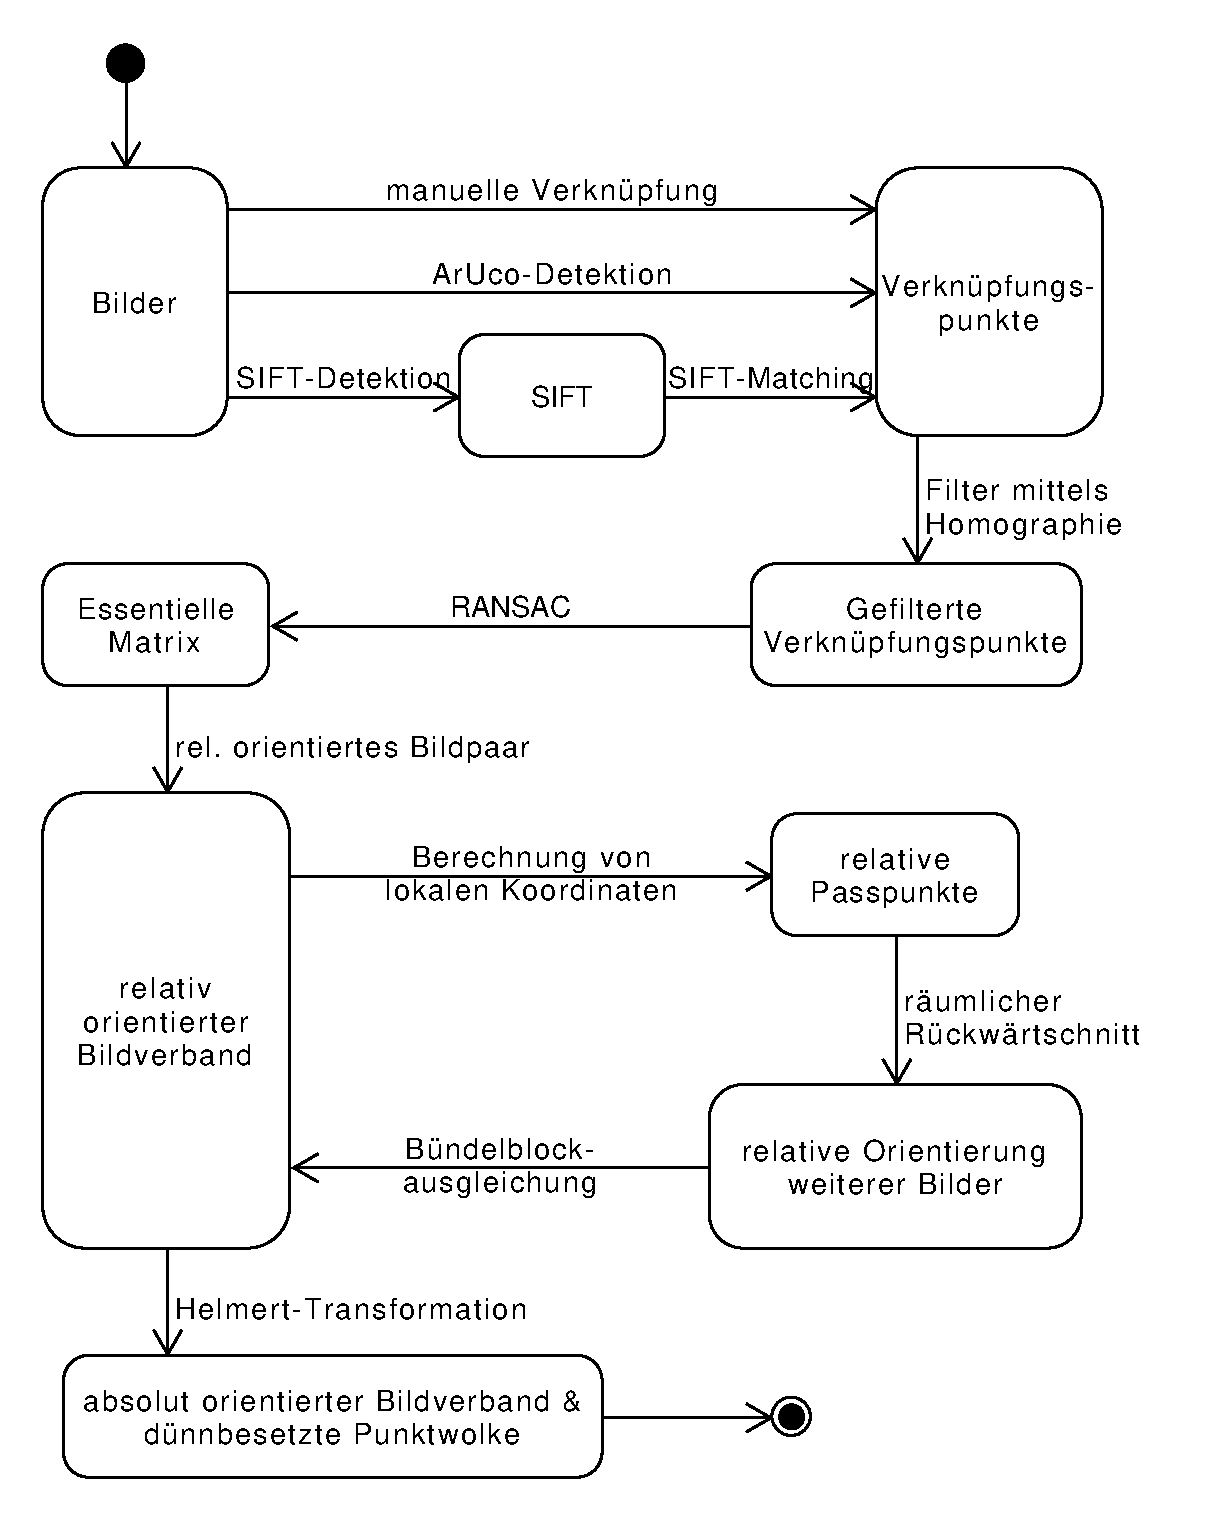
\includegraphics[width=0.8\textwidth]{./img/Ablauf.pdf}
\centering
 \caption{Ablauf der Bildverknüpfung} %Bildunterschrift
 \label{img:ablauf} %ID fürs Bild
\end{figure}

\section{Bilder}
Die Berechnung der Tiefeninformationen ist bei Structure-from-Motion nur möglich aufgrund der Bewegung der Kamera zwischen den Bildern. Um möglichst gute Schnitte zur Verfügung zu haben und die innere und äußere Orientierung möglichst gut berechnen zu können, müssen diese Bilder einige Bedingungen erfüllen.

\subsubsection{Kameraeinstellungen}
Jede Einstellung der Kameraoptik verändert die innere Orientierung und auch jede Kamera (auch einer Modellreihe) ist unterschiedlich. Daher sollten die Bilder möglichst mit einer Kamera mit festen Einstellungen (Brennweite, Blende, Objektiv) aufgenommen werden. Bei der Empfindlichkeit (ISO-Zahl) oder Belichtungszeit wären Änderungen unproblematisch für die innere Orientierung und bei sich stark ändernden Helligkeitsverhältnissen auch hilfreich, jedoch wird hierdurch auch die Helligkeit der Verknüpfungspunkte verändert, was wiederum problematisch sein kann. Entsprechend ist es empfehlenswert bei gleichmäßiger Beleuchtung, die sich auch nicht ändern sollte, die Bilder zu erstellen - also beispielsweise bei bedeckten Himmel.

\subsubsection{Überlappung und Bildinhalte}
Da die Bilder durch identische Punkte verbunden werden, müssen die Bildinhalte sich überlappen. Außerdem sollten alle Bilder strukturierte Bereiche aufweisen. \citep[S. 146f]{opendronemap}

\subsubsection{Bewegungen der Kamera}
Bilder, die vom gleichen Standpunkt aufgenommen wurden, sind oft nur ungenau verknüpfbar. Daher empfiehlt es sich, eher um Objekte herum zu gehen, statt beispielsweise bei Innenräumen sich nur in die Mitte zu stellen und sich zu drehen. Während der Aufnahmen sollte die Kamera natürlich möglichst ruhig gehalten werden, um möglichst scharfe Bilder zu generieren. Dies ist vor allem bei UAV-Flügen relevant, die auch aus hoher Geschwindigkeit Bilder aufnehmen könnten. Jedoch weisen die meisten Digitalkamera einen Rolling-Shutter-Effekt auf, dass heißt die Bildreihen werden nicht alle zeitgleich aufgenommen, sondern die oberen vor den unteren. Daher ist es sinnvoll, das UAV kurz schweben zu lassen und dann ein Bild zu machen. \citep[S. 147]{opendronemap}

\subsubsection{Abstand bzw. Höhe}
Umso weiter die Kamera vom Objekt entfernt ist, umso mehr Inhalte und entsprechend mehr Verknüpfungsmöglichkeiten sind im Bild enthalten. Daher sollte sich immer klar gemacht werden, welche Auflösung benötigt wird und entsprechend die Entfernung bzw. bei UAV-Aufnahmen die Höhe zu wählen. Der Abstand sollte außerdem variiert werden, da dieses bei der Ausgleichung der inneren Orientierung hilft. \citep[S. 144f]{opendronemap}


\section{Verknüpfungspunkte}
Um die einzelnen Bilder verknüpfen zu können, werden identische Punkte zwischen zwei oder mehr Bildern benötigt. Diese können klassisch per Hand erfasst werden, jedoch ist dieses schon bei kleineren Projekten sehr zeitaufwändig. Daher wurde zusätzlich die Möglichkeit genutzt, automatisch Verknüpfungspunkte zu erzeugen.

\subsection{ArUco-Marker}
Eine Variante der automatischen Verknüpfungspunkte sind die sogenannten ArUco-Marker. Diese werden häufig für die Orientierung bei Augmented-Reality-Anwend\-ungen genutzt. OpenCV unterstützt die Erkennung dieser Marker. Sie werden als codierte Messmarken verwendet und können automatisch im Subpixelbereich erkannt werden. Jede Ecke kann hier einzeln identifiziert werden, sodass ein erkannter Marker vier Verknüpfungspunkte liefern kann.

\subsection{SIFT}
Die SIFT-Methode liefert Verknüpfungspunkte aus Mustern auf den fotografierten Oberflächen. Es ist meist nicht notwendig explizit Marker an dem aufzunehmenden Objekt anzubringen, sofern seine Oberfläche nicht strukturlos ist (glatte weiße Wände etc.) oder in Bewegung ist.

Zur Erkennung von Merkmalen setzt das Verfahren auf die Detektion von Kanten. Diese werden in verschiedenen Stufen einer Bildpyramide erkannt und ihre Extrema berechnet. Es werden diese Merkmale weiter ausgedünnt, beispielsweise über den Kontrast. Sofern ein möglicher Marker identifiziert wurde, wird eine Beschreibung erzeugt. Diese erfolgt  durch Analyse der Helligkeitsabweichungen zu den Nachbar-Pixeln und wird an der stärksten Abweichung ausgerichtet. Hierdurch wird die Beschreibung dann richtungsunabhängig. Mit diesen kann dann die Übereinstimmung von zwei Markern in zwei Bildern bestimmt werden, auch wenn die Bilder zueinander gekippt oder gedreht sind.
\citep[S. 483]{luhmann}

\section{Verknüpfung von Bildern}
\label{s:photogramm}
Durch die drei beschriebenen Verfahren und die hieraus entstandenen Verknüpfungs\-punkte können die Bilder miteinander verknüpft werden. Da durch GNSS nur eine sehr grobe und ggf. auch falsche Vorausrichtung besteht, kann diese nur als sehr grobes Hilfsmittel genutzt werden. In diesen Ansatz wird es nur für die Beschränkung der SIFT-Detektion auf Bilder, die nahe beieinander sind oder sich ArUco- oder manuelle Punkte teilen, genutzt.
Für die eigentliche Verknüpfung werden dann nur photogrammmetrische Verfahren genutzt. Über diese wird im Folgenden ein kurzer Überblick gegeben.

\begin{comment}
\subsection{Homographie}
grobe Filterung
\end{comment}

\subsubsection{Abbildungsgleichung}
\label{ss:abbildungsgleichung}
Die Abbildung eines Punktes auf einem Bild wird durch die Abbildungsgleichung beschrieben. In der Matrizenrechnung ergibt sich dieser aus der Multiplikation mit der Projektionsmatrix $P$. Diese ergibt sich aus der Kameramatrix $K$, der Rotation $R$ und dem Projektionszentrum $X_0$. (siehe \autoref{abbildungsgleichung}, nach \citealp[S. 244]{hartley} und \citealp[S. 288]{luhmann})

\begin{align}
\label{abbildungsgleichung}
    x' &= P \cdot X\\
    P &= K \cdot [R|X_0] \\
    P &= 
    \begin{bmatrix}
    c_x & 0 & x'_0 \\
    0 & c_y & y'_0 \\
    0 & 0 & 1
    \end{bmatrix} \cdot \begin{bmatrix}
    r_11 & r_21 & r_31 & X_0 \\
    r_12 & r_22 & r_32 & Y_0 \\
    r_13 & r_23 & r_33 & Z_0 \\
    \end{bmatrix} 
\end{align}

Um die Beziehung zwischen zwei Bildern aufzustellen, kann man die Abbildungsgleichung nutzen. Da es hier nur um die Beziehung zwischen zwei Bildern geht, kann die Rotation und Translation des ersten Bildes auf 0 gesetzt werden ($R$ ist dann eine 3x3-Einheitsmatrix und $X_0$ ein Nullvektor). $X_0$ des zweiten Bildes wird zur Translation zwischen den beiden Bildern. \citep[S. 326]{luhmann}

\subsubsection{Fundamental-/Essentielle Matrix}
Die Fundamentalmatrix beschreibt das Verhältnis von identischen Punkten in zwei Bildern zueinander. Sie kann genutzt werden, um die Drehung und Verschiebung zwischen zwei Aufnahmeorten zu bestimmen. Die Formel für die Fundamentalmatrix lautet:
\begin{align}
x'^T \cdot F \cdot x'' &= 0
\end{align}
Sie unterscheidet sich nur von der Essentiellen Matrix in der Eigenschaft, dass bei der Essentiellen Matrix die Kameraparameter bekannt sein müssen. Diese werden dann auf die Bildkoordinaten angewendet und $x'$ und $x''$ werden so unabhängig (normalisiert) von den Kameraeinstellungen. Mittels Singulärwertzerlegung lässt sich dann die Rotation und Translation aus der Essentiellen Matrix bestimmen. Im Falle von Bildern die mit Digitalkameras aufgenommen wurden sind die Kameraparameter zumindest näherungsweise aus den EXIF-Daten der Bilder bekannt, sodass dieser Weg hier genutzt werden kann. \citep[S. 257]{hartley}

In der entstandenen Software wurde die Methode verwendet, um die Verknüpfung des Startpaares zu errechnen.

\subsection{Fundamental-/Essentielle Matrix}
Die Fundamentalmatrix beschreibt das Verhältnis von identischen Punkten in zwei Bildern zueinander. Sie kann genutzt werden, um die Drehung und Verschiebung zwischen zwei Aufnahmeorten zu bestimmen. Die Formel für die Fundamentalmatrix lautet:
\begin{align}
x'^T \cdot F \cdot x'' &= 0
\end{align}
Sie unterscheidet sich nur von der Essentiellen Matrix in der Eigenschaft, dass bei der Essentiellen Matrix die Kameraparameter bekannt sein müssen. Diese werden dann auf die Bildkoordinaten angewendet und $x'$ und $x''$ werden so unabhängig (normalisiert) von den Kameraeinstellungen. Mittels Singulärwertzerlegung lässt sich dann die Rotation und Translation aus der Essentiellen Matrix bestimmen. Im Falle von Bildern die mit Digitalkameras aufgenommen wurden sind die Kameraparameter zumindest näherungsweise aus den EXIF-Daten der Bilder bekannt, sodass dieser Weg hier genutzt werden kann. \citep[S. 257]{hartley}

In der entstandenen Software wurde die Methode verwendet, um die Verknüpfung des Startpaares zu errechnen.

\subsection{Vorwärtsschnitt}
Aus den zwei Projektionsmatrizen zweier Bilder und der Position eines identischen Punktes in beiden Bildern lassen sich dann lokale (Modell-)Koordinaten des Punktes berechnen. Da auch dieses nicht fehlerfrei ist, wurde hierfür die Methode der linearen Triangulation verwendet. Hierbei wird der entstehende Fehler ausgeglichen. \citep[S.312]{hartley}

\subsection{Rückwärtsschnitt}
Entsprechend lässt sich auch aus der Position von Punkten mit bekannten lokalen Koordinaten die Position und Drehung eines Bildes berechnen. Dieses wurde genutzt, um weitere Bilder an das Startpaar heranzuknüpfen. Hierfür werden mindestens 5 Punkte benötigt. \citep[S. 533ff]{hartley}


\section{Bündelblockausgleichung}
Mittels Bündelblockausgleichung können die grob mit den vorher genannten Verfahren bestimmten Positionen und Drehungen in einer Ausgleichung optimiert werden. Hierzu gehen alle Parameter der Bilder und die Positionen der Passpunkte in die gemeinsame Ausgleichung ein. Grundlage der Ausgleichung ist die in \autoref{ss:abbildungsgleichung} beschriebene Abbildungsgleichung. Als Ergebnis erhält man die ausgeglichenen Parameter und Genauigkeitsangaben für diese. \citep[S. 340]{luhmann}

\section{Transformation}
Die Berechnungen erfolgen alle in einem lokalen Koordinatensystem. Die GNSS-Koordi\-naten der Bilder werden nur genutzt, um potentielle Nachbarbilder zu identifizieren. Daher muss zum Schluss eine 3D-Transformation der lokalen Daten in ein weltweites Koordinatensystem erfolgen. Diese Transformation erfolgt erst in ein geozentrisches, kartesisches Koordinatensystem (ECEF), welches dann in Längen- und Breitengrade sowie Höhen über dem Ellipsoid umgerechnet werden. Die letztgenannten Angaben sind für die EXIF-Daten der Bilder notwendig.

\chapter{Aufbau des Messystemes}

\chapter {Software-Entwicklung}
Die Entwicklung erfolgte mittels Prototyping. Die einzelnen Arbeitspakete wurden als eigenständige Jupyter-Notebooks programmiert und jeweils immer weiter bis zu der gewünschten Funktionalität entwickelt. Anschließend wurden die einzelnen Module zu einem Gesamtprogramm zusammengeführt und eine Weboberfläche zur Steuerung und Kontrolle erzeugt. Auf die einzelnen Problemstellungen wird im \autoref{ss:vorgehen} eingegangen.

\section{Konzeption}

Entsprechend der benötigten Schritte aus \autoref{c:photogrammmetrie} und \autoref{img:ablauf} wurde die Anwendungsfälle, die die Benutzeroberfläche ermöglichen soll, im Anwendungsfall-Diagramm in \autoref{img:anwendungsfall} zusammengetragen.

\begin{figure}[!htbp]
 \centering
 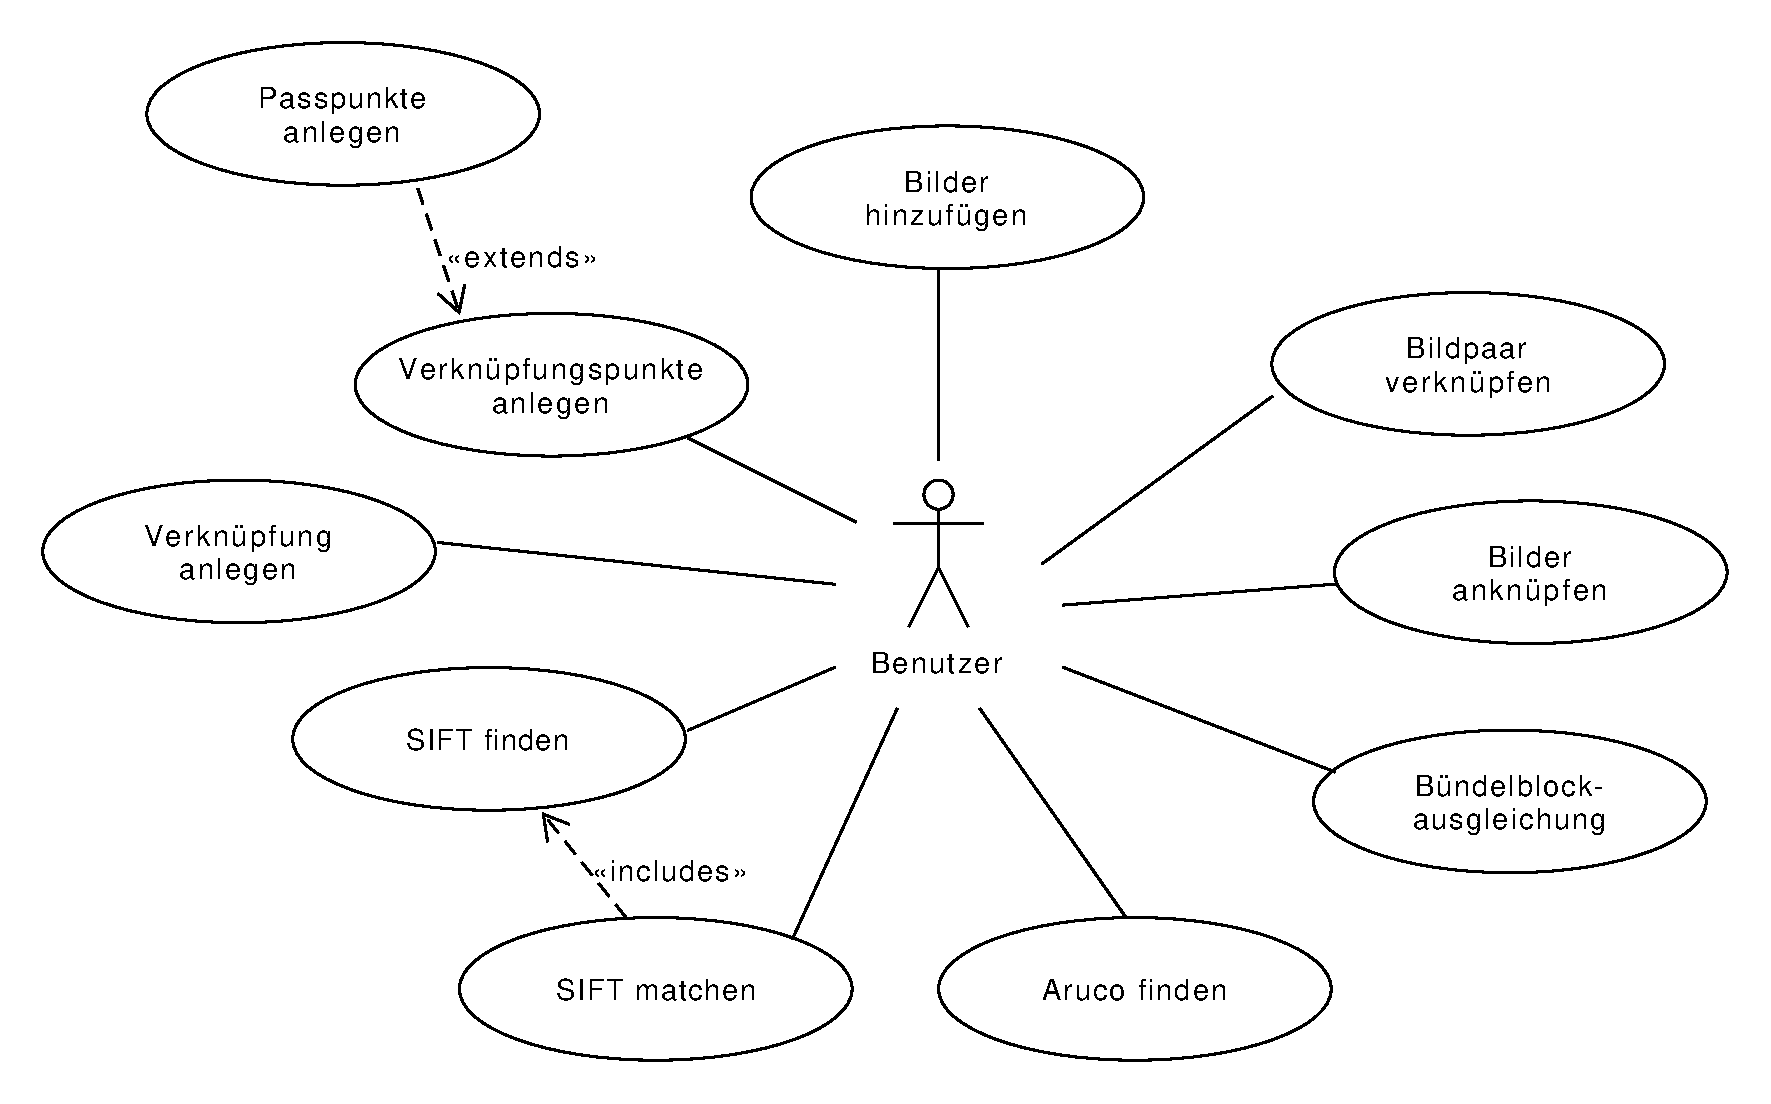
\includegraphics[width=1\textwidth]{./img/UseCase.pdf}
\centering
 \caption{Anwendungsfall-Diagramm} %Bildunterschrift
 \label{img:anwendungsfall} %ID fürs Bild
\end{figure}

Aus den benötigten Daten wurde das Domänen-Klassendiagramm aus \autoref{img:dokladia} erzeugt. Dieses zeigt vor allem die Abhängigkeiten der einzelnen Datensätze untereinander.

\begin{figure}[!htbp]
 \centering
 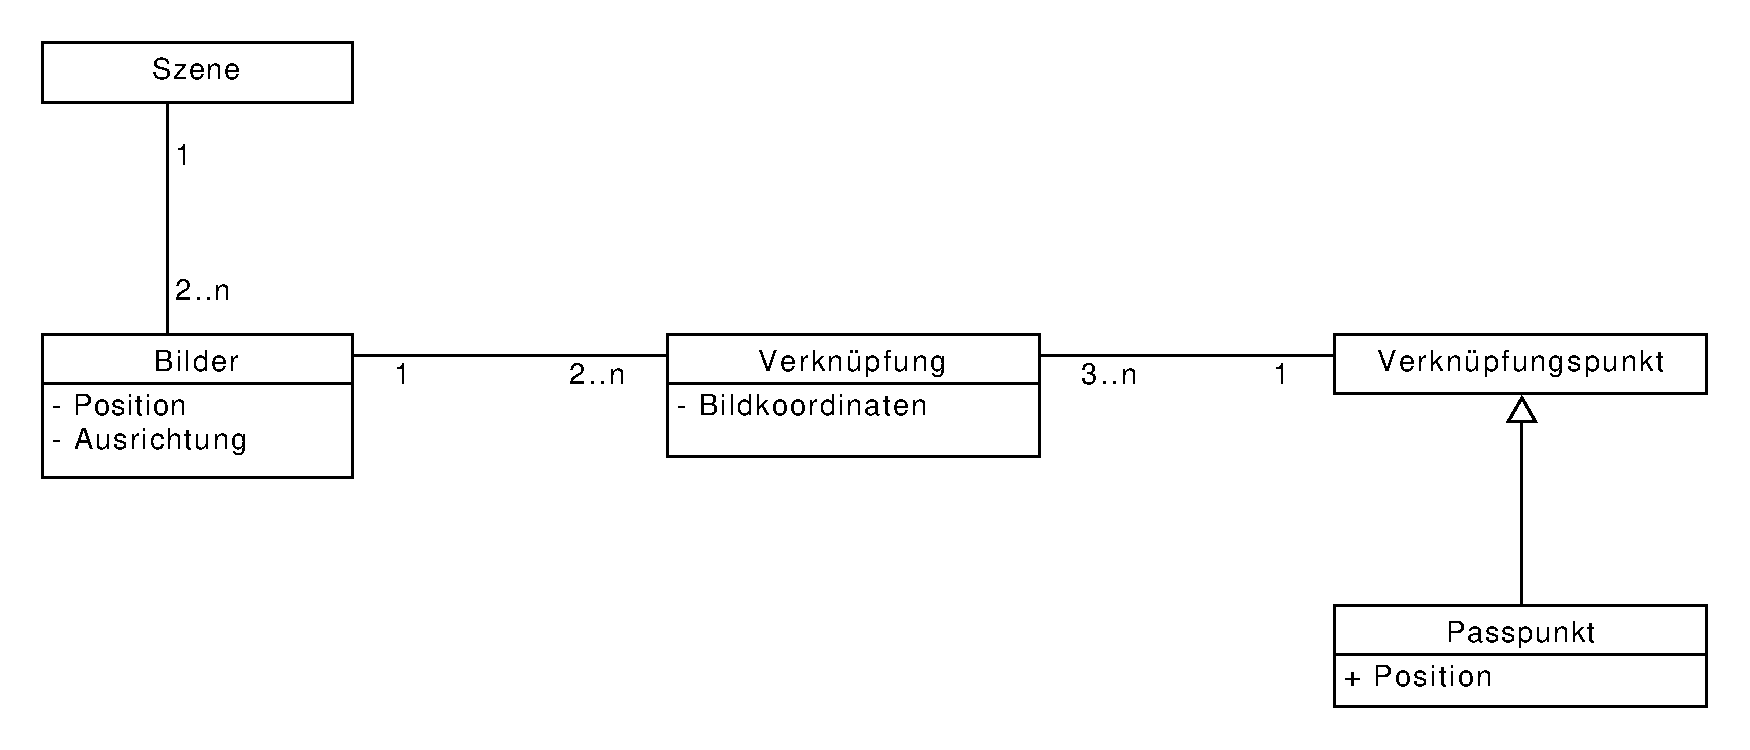
\includegraphics[width=1\textwidth]{./img/DomaenenKlassendiagramm.pdf}
\centering
 \caption{Domänen-Klassendiagramm} %Bildunterschrift
 \label{img:dokladia} %ID fürs Bild
\end{figure}

\section{Implementierung}
Dieses ist dann auch Grundlage für die Implementierung der SQLite-Datenbank. Der Datenbankaufbau ist \autoref{img:datenbank} zu entnehmen. Die Datenbank dient der Zwischenspeicherung der Passpunkte und der durchgeführten Berechnungen. 

\begin{figure}[!htbp]
 \centering
 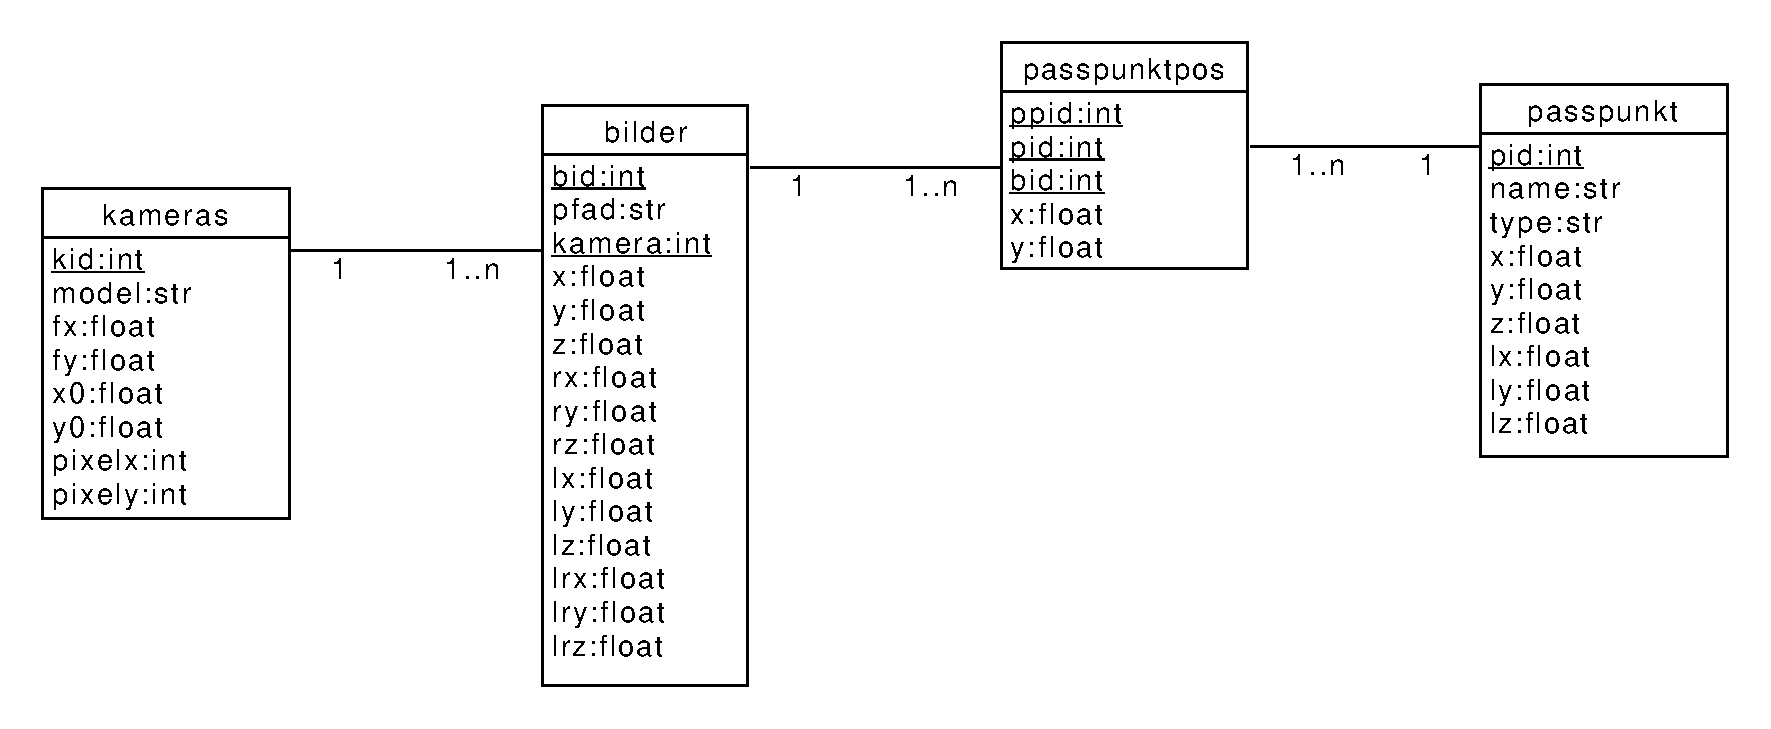
\includegraphics[width=1\textwidth]{./img/datenbank.pdf}
\centering
 \caption{Datenbank-Struktur} %Bildunterschrift
 \label{img:datenbank} %ID fürs Bild
\end{figure}

Das Backend wurde in Python entwickelt. Die Pakete orientieren sich an den Arbeitsschritten aus dem Ablaufdiagramm (\autoref{img:ablauf}). Die einzelnen Python-Module greifen auf die oben beschriebene SQLite-Datenbank zu. Die einzelnen Module sind der Übersicht in \autoref{img:python} zu entnehmen.

\begin{figure}[!htbp]
 \centering
 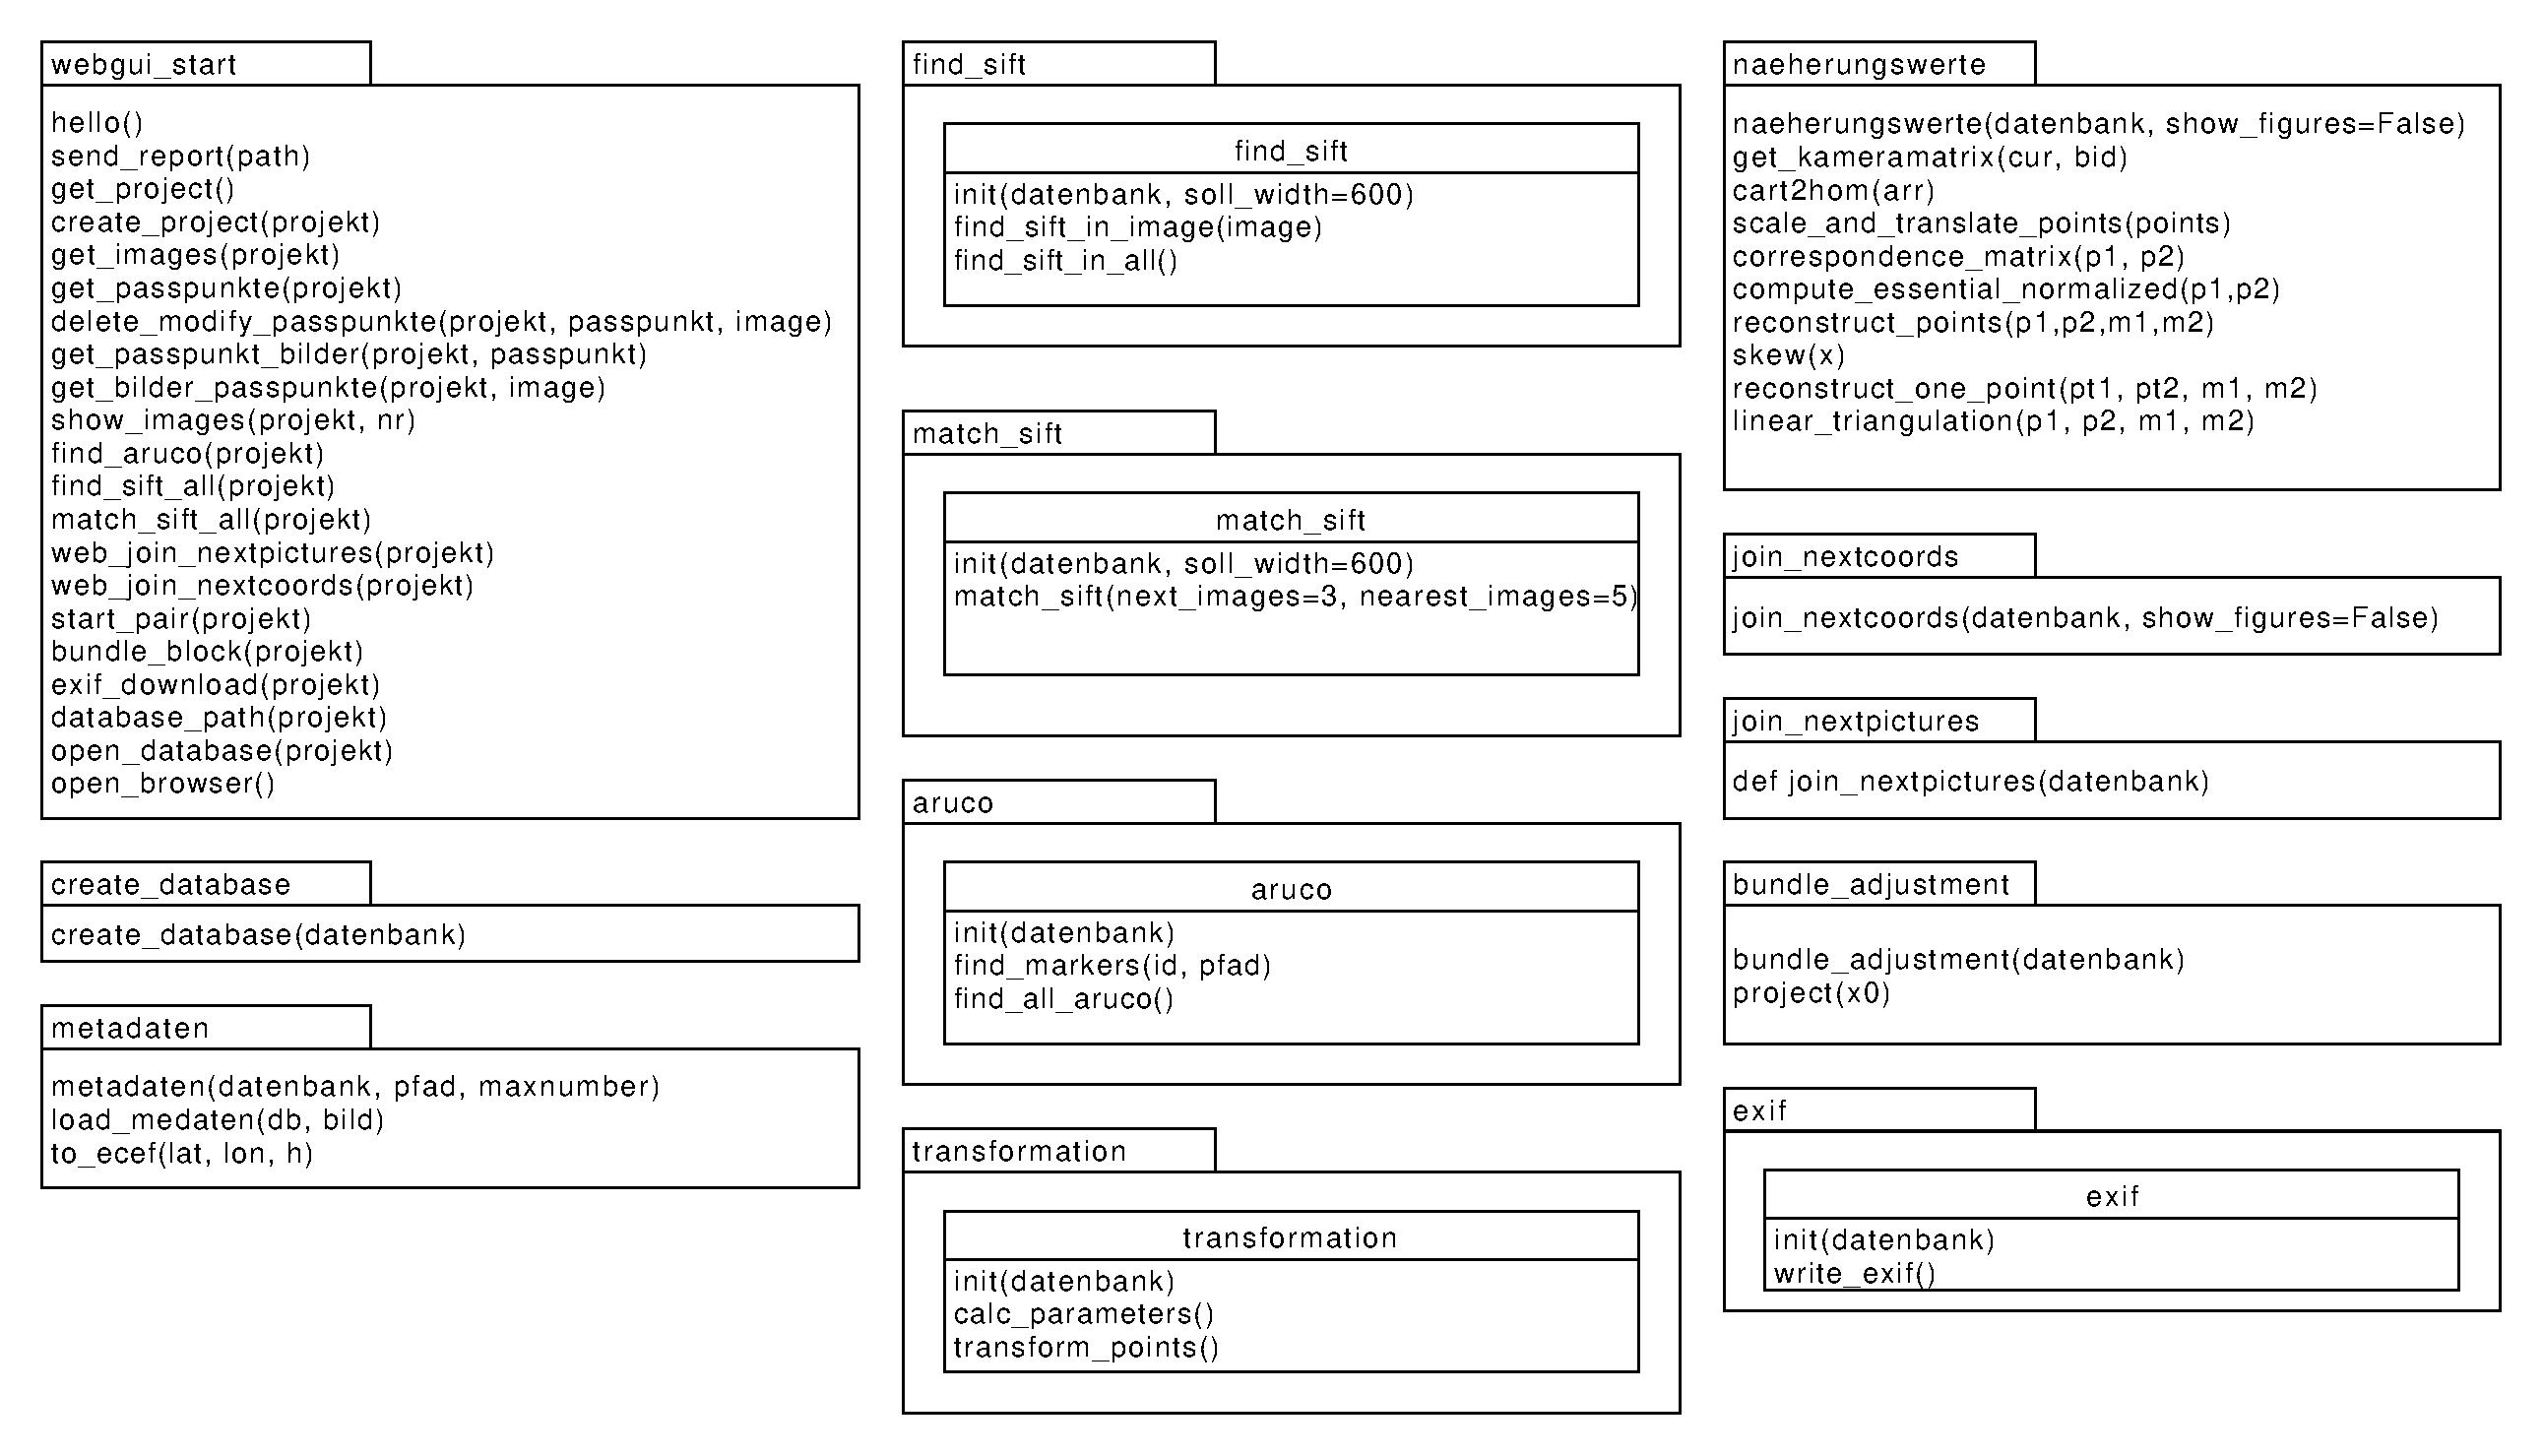
\includegraphics[width=1\textwidth]{./img/python.pdf}
\centering
 \caption{Implementierung der Python-Pakete} %Bildunterschrift
 \label{img:python} %ID fürs Bild
\end{figure}

Über das Webstart-Modul werden dann die einzelnen Module über eine Website mit TypeScript angesprochen. Die einzelnen TypeScript-Klassen sind der \autoref{img:typescript} zu entnehmen. Hierbei wurde darauf Wert gelegt, die einzelnen Funktionen modular zu halten, sodass die Möglichkeit besteht, das System mit weiteren Modulen zu erweitern.

\begin{figure}[!htbp]
 \centering
 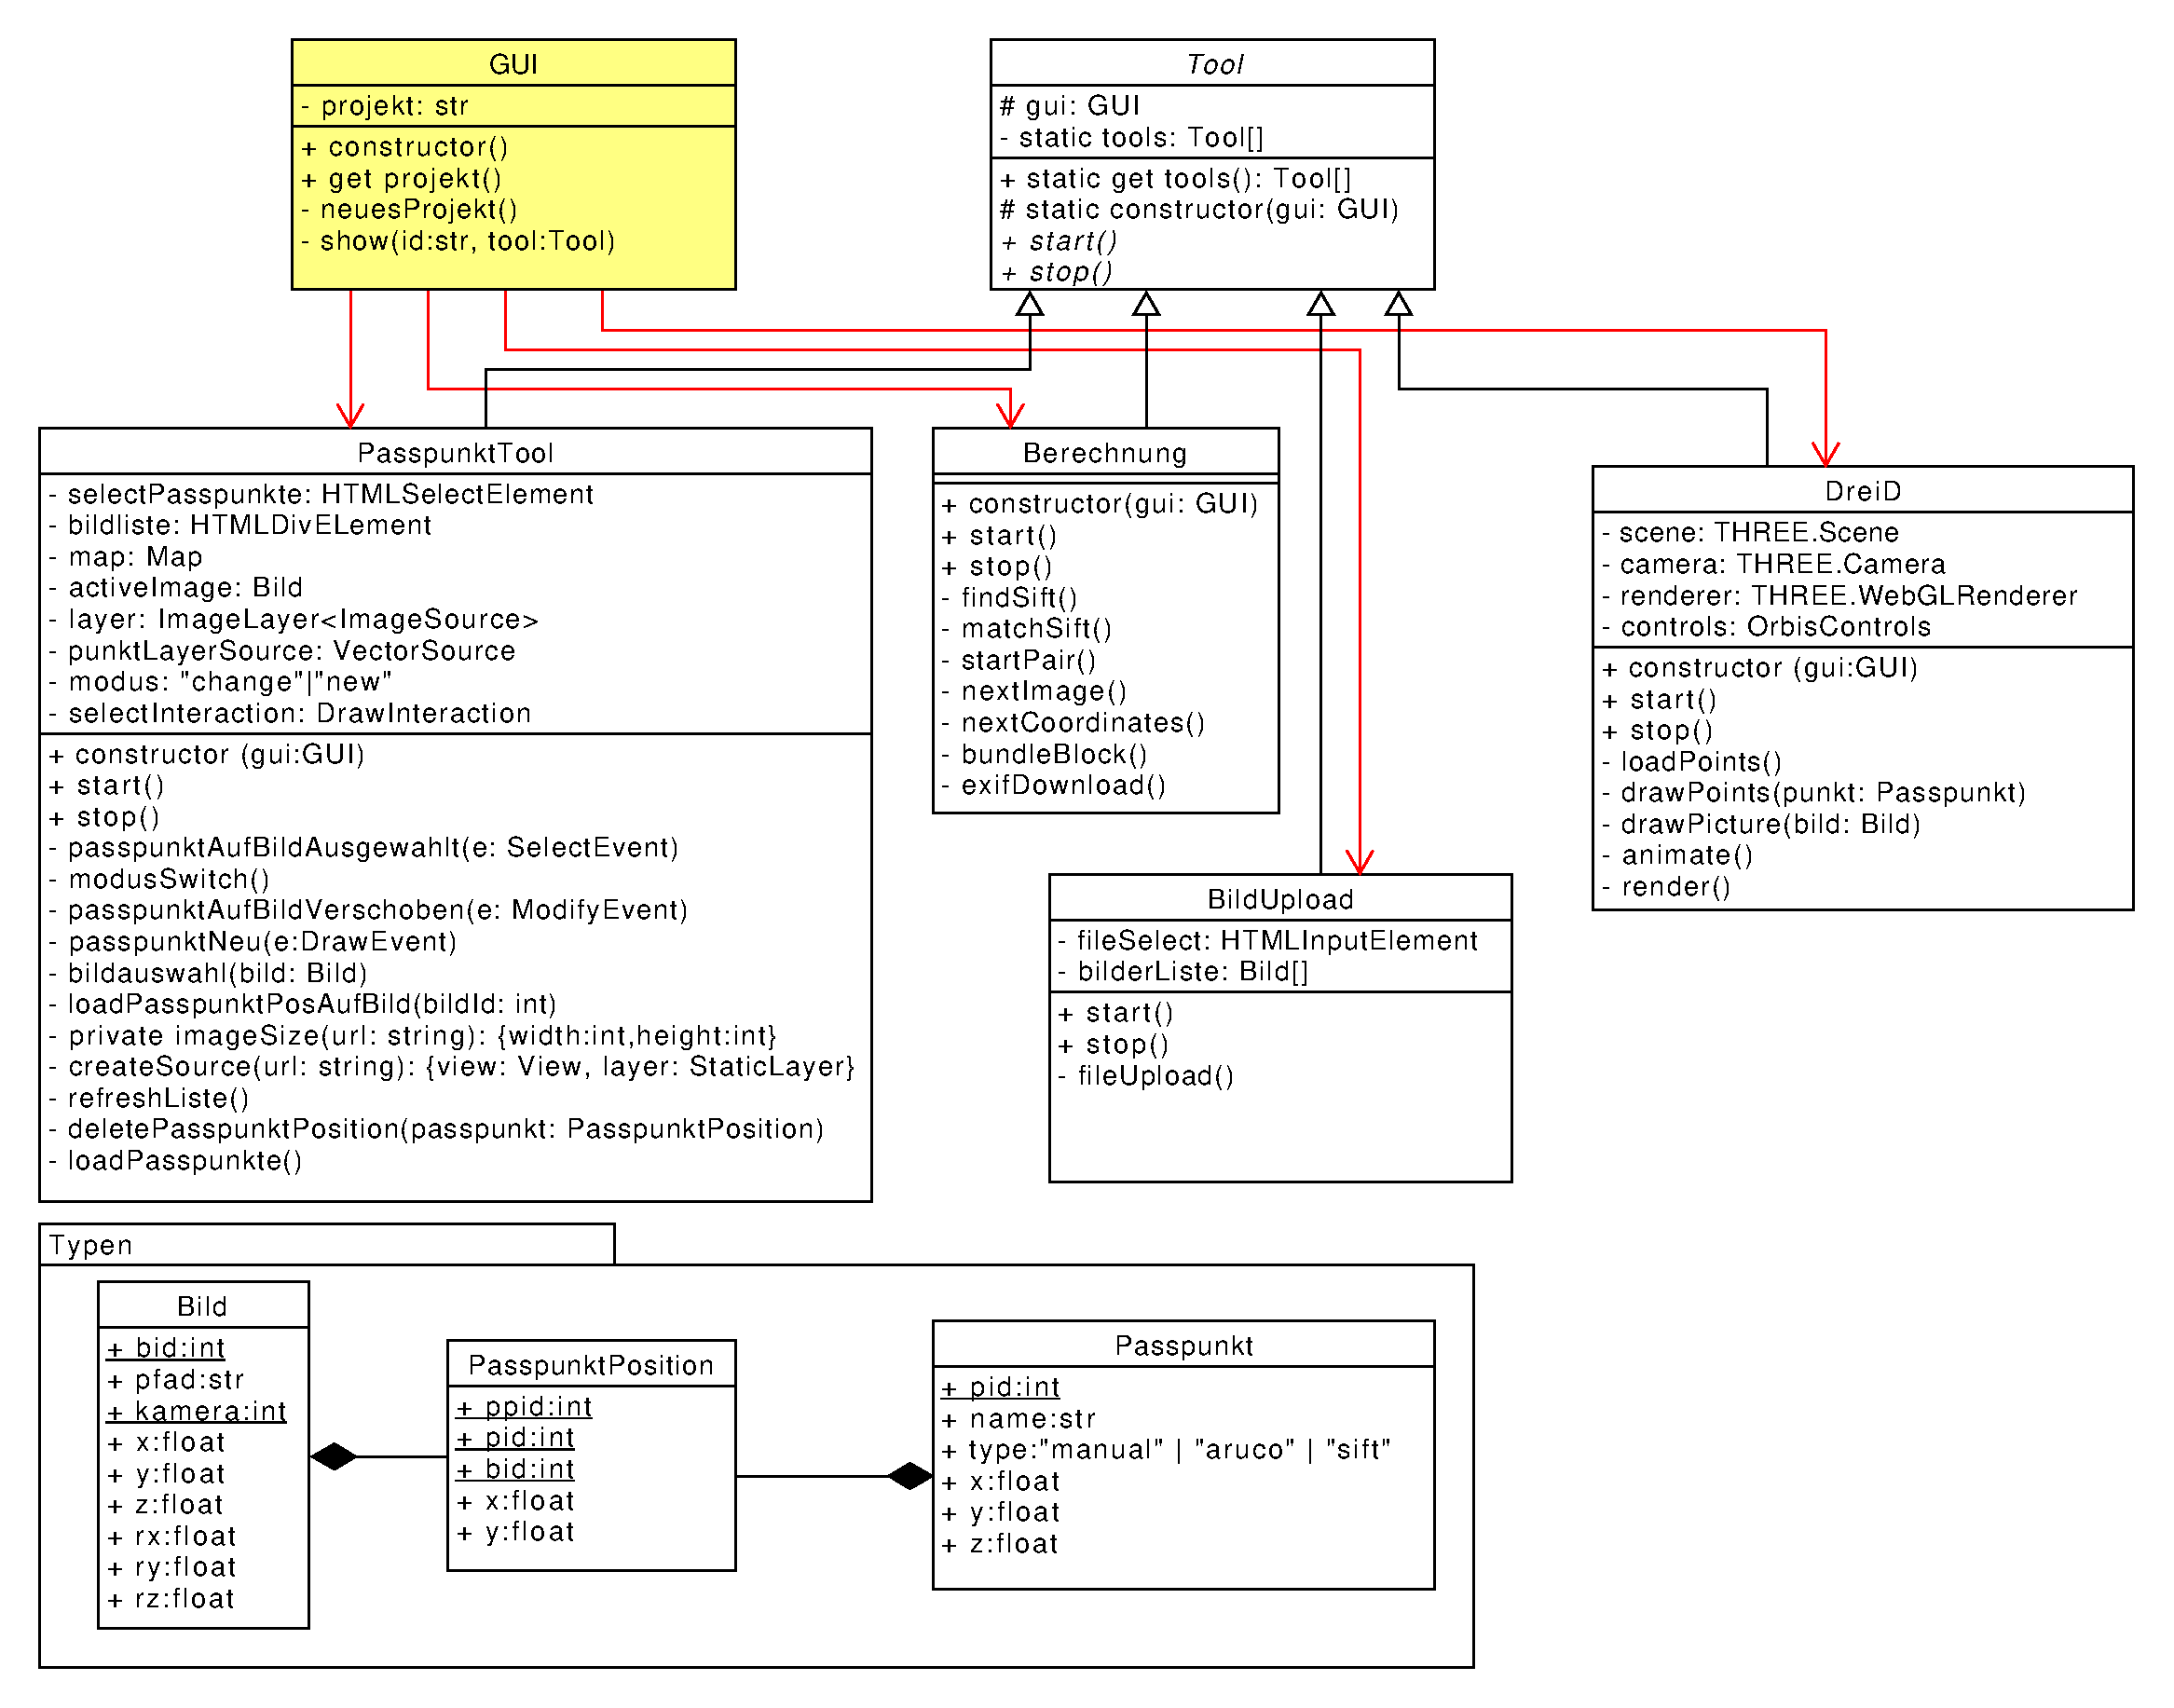
\includegraphics[width=1\textwidth]{./img/typescript.pdf}
\centering
 \caption{Implementierung der TypeScript-Klassen} %Bildunterschrift
 \label{img:typescript} %ID fürs Bild
\end{figure}



\section{Vorgehen}
\label{ss:vorgehen}

Die Programmierung des Systemes erfolgte iterativ. Einzelne Arbeitspakete wurden in einem Jupyter-Notebook ausprobiert und dann, wenn dieser Schritt erfolgreich war, in den Gesamtworkflow integriert. Größtenteils wurden der Python-Code objektorientiert und typisiert geschrieben, einzelne Module sind jedoch noch aus der Prototyp-Phase funktionsbasierend programmiert.

\subsection{Python-Bibliotheken}
Es wurde, wenn möglich, auf Python-Bibliotheken zurückgegriffen. Hierdurch sollte der Programmieraufwand verringert und auf bereits getesteten Code gesetzt werden. Wo dieses nicht möglich war, wurden Funktionen entsprechend Code-Beispielen aus GitHub oder \glqq Rezepten\grqq{} aus dem Werk von \citeauthor{hartley} programmiert. 

\subsubsection{OpenCV} ist eine Bibliothek für Bildbearbeitung und maschinelles Sehen. Sie ist weit verbreitet und bietet viele photogrammetrische Funktionen. Viele der unter \autoref{s:photogramm} beschriebenen Schritte wurden mit dieser Bibliothek durchgeführt. \citep{opencv} Es zeigten sich jedoch Probleme bei der Berechnung der Essentiellen Matrix, sodass diese mit Hilfe eines Codebeispieles von \cite{3drec} auf Grundlagen von \cite{hartley} berechnet wurde.

\subsubsection{NumPy} bietet neben vielen weiteren Funktionen die Möglichkeit der Matrizenrechnung. Diese wurde für viele Berechnungen benötigt.

\subsubsection{SciPy} wurde für die Berechnung der Bündelblockausgleichung verwendet. Der manuelle Ansatz mit den Formeln aus \cite{luhmann} unter Nutzung von NumPy war sehr ressourcenlastig. Unter Verwendung von SciPy und der Projektionsgleichung konnte die Berechnungsdauer stark dezimiert werden.

\subsubsection{Flask} wurde genutzt um die Weboberfläche bereitzustellen und die Kommunikation zwischen dem Python und dem HTML/TypeScript-Modulen sicherzustellen. Die Weboberfläche selber muss nur einmalig kompiliert werden und wird dann von einen Flask-Webserver zur Verfügung gestellt. Per REST-Abfragen werden dann Daten zwischen TypeScript (bzw. nach dem Kompilieren eigentlich JavaScript) und Python ausgetauscht.

\subsubsection{OpenSFM} wurde zwischenzeitlich verwendet um photogrammetrische Berechnung durchzuführen. Jedoch wurde dieses aufgrund mangelnder Anpassungsmöglichkeiten wieder verworfen. OpenSFM basiert aber auch unter anderem auf OpenCV. Der Code von OpenSFM wurde in der Prototyping-Phase zur Ideenfindung genutzt.

Erstaunlicherweise wurde kein brauchbares Paket zur Durchführung einer Helmert-Transformation mittels identischer Punkte gefunden. Daher wurde hier eine Funktion geschrieben, die eine Abbildungsmatrix mit Hilfe der Methode der kleinsten Quadrate errechnet. Nachteilig ist bei dieser Lösung jedoch, dass diese Ausgleichung auch Scherungen und unterschiedliche Maßstäbe für die einzelnen Koordinatenkomponenten unterstützt. Eigentlich wäre jedoch eine Transformation mit einem festen Maßstab sinnvoller, da die errechnete Struktur durch die Bündelblockausgleichung bereits deutlich besser der Realität entspricht als die GNSS-Koordinaten, die zur Transformation genutzt wurden. So werden die Daten aktuell an dieser Stelle wieder verschlechtert.

\subsection{TypeScript/JavaScript-Module}
Wie bereits erläutert wurde die GUI in Form einer Webseite entwickelt. Entsprechend wurden hier JavaScript-Module verwendet. Da TypeScript durch seinen Kompiler wieder zu JavaScript umgeformt wird, kann hier auch auf die große Auswahl von JavaScript-Bibliotheken aus dem Node Package Manager zurückgriffen werden.

\subsubsection{OpenLayers} ist eigentlich zur Anzeige von Online-Karten gedacht. In diesem Fall wurde es zur Darstellung der Passpunkte auf den Bildern genutzt. Es bietet einfache und weitläufig bekannte Funktionen zum Zoomen und Digitalisieren. Statt einer Karte wurde in dem entsprechenden Fenster das Bild und die Passpunkte als Marker auf diesem visualisiert. Auch die Editierfunktionen wurden hieraus genutzt.

\subsubsection{Three.JS} ist eine Bibliothek zur Darstellung von 3D-Inhalten. Diese wurde hier genutzt um eine Vorschau der errechneten 3D-Koordinaten bereitzustellen.


\chapter{Ausblick und Fazit}
Vor allem das Erzeugen der Näherungswerte in Vorbereitung der Bündelblockausgleich\-ung benötigte deutlich mehr Zeit und Theorieverständnis als gedacht. Daher wurde leider nicht alle ursprünglich geplanten Features umgesetzt. Aufgrund von Krankheit und anderen Uni-Projekten konnte dann zusätzlich auch nicht so viel Zeit in der zweiten Semesterhälfte in das Projekt gesteckt werden, wie eigentlich ursprünglich gedacht. Es sind bisher beispielsweise keine Nebenbedingungen möglich - ein Festlegen eines Maßstabes aufgrund einer bekannten Strecke ist so nicht möglich und auch nicht die Optimierung der Ausrichtung durch die Angabe gleich hoher Punkte. Auch wird aktuell nur die Position, nicht jedoch die bereits errechnete Drehung in den EXIF-Daten gespeichert. Hierfür müsste noch eine Umrechnung der Drehung aus dem System der ECEF-Koordinaten in die für EXIF-Daten übliche Ausrichtung an der Lotrichtung der Ortes des Bildes erfolgen. Ein weiteres offenes Problem ist die bereits erwähnte Transformation des lokalen Koordinatensystemes. Hier müsste noch die Ausgleichung so optimiert werden, dass nur ein Maßstab und keine Scherung verwendet wird.

Neben den erwähnten fehlenden Funktionen wäre als weitere Erweiterungen eine Berechnung einer dichten Punktwolke denkbar. Entsprechende Bibliotheken wurden währ\-end der Entwicklung entdeckt und schienen relativ leicht einbaubar. So würde die Software zu einer Komplettlösung für Structure-from-Motion-Punktwolken aus Bildern werden. 

Im Gesamten sorgte das Projekt dafür, ein tiefergehendes Verständnis von Photogrammmetrie im Allgemeinen und Structure-from-Motion im Speziellen zu erarbeiten sowie vor allem die Probleme und Schwierigkeiten kennenzulernen.
\clearpage
%Literatur
\renewcommand\UrlFont\itshape
\renewcommand{\refname}{Literaturverzeichnis}
\bibliography{photoBox}
%\printbibliography
\listoffigures
\listoftables
%\lstlistoflistings

\end{document}